%% packages
\documentclass{article}
\usepackage[a4paper, left=2.0cm, right=2.0cm, top=3.5cm]{geometry}
\usepackage[ngerman]{babel}
\usepackage{graphicx}
\usepackage{multicol}
\usepackage{amssymb}
\usepackage{titlesec}
\usepackage{wrapfig}
\usepackage{blindtext}
\usepackage{lipsum}
\usepackage{caption}
\usepackage{listings}
\usepackage{fancyhdr}
\usepackage{nopageno}
\usepackage{authblk}
\usepackage{amsmath} % tons of math stuff
\usepackage{mathtools} % e.g. alignment within matrix
%\usepackage{bm} % provides shorthand for bold in math mode
\usepackage{dsfont} % \mathds makes double stroke digits
\usepackage{esdiff} % provides \diff
%\usepackage[ISO]{diffcoeff}
\usepackage{xcolor}
\usepackage{csquotes} % e.g. provides \enquote
\usepackage[separate-uncertainty=true]{siunitx} % units
\usepackage{xcolor} % colored text
\usepackage{csvsimple}
\usepackage{subcaption}
\usepackage{physics}
\usepackage{hyperref}
\usepackage{nameref}
\hypersetup{colorlinks=true, linkcolor=black, pdfhighlight={/N}}
\usepackage{tcolorbox}
\usepackage{amsthm}




%\fancyhf[]{}

%% custom stuff
% own units
\DeclareSIUnit \VSS {\ensuremath{V_\mathrm{SS}}}
\DeclareSIUnit \VS {\ensuremath{V_\mathrm{S}}}
\DeclareSIUnit \Veff {\ensuremath{V_\mathrm{eff}}}
\DeclareSIUnit \Vpp {\ensuremath{V_\mathrm{pp}}}
\DeclareSIUnit \Vp {\ensuremath{V_\mathrm{p}}}
\DeclareSIUnit \VRMS {\ensuremath{V_\mathrm{RMS}}}
\DeclareSIUnit \ASS {\ensuremath{A_\mathrm{SS}}}
\DeclareSIUnit \AS {\ensuremath{A_\mathrm{S}}}
\DeclareSIUnit \Aeff {\ensuremath{A_\mathrm{eff}}}
\DeclareSIUnit \App {\ensuremath{A_\mathrm{pp}}}
\DeclareSIUnit \Ap {\ensuremath{A_\mathrm{p}}}
\DeclareSIUnit \ARMS {\ensuremath{A_\mathrm{RMS}}}

% change subsection numbering to capital letters
\newcommand{\subsectionAlph}{ \renewcommand{\thesubsection}{\arabic{section}.\Alph{subsection}} }
% change subsection numbering to lowercase letters
\newcommand{\subsectionalph}{ \renewcommand{\thesubsection}{\arabic{section}.\alph{subsection}} }
% change subsubsection numbering to lowercase letters
\newcommand{\subsubsectionalph}{ \renewcommand{\thesubsubsection}{\arabic{section}.\arabic{subsection}.\alph{subsubsection}} }
% own fig. that works with multicols
\newenvironment{Figure}
  {\par\medskip\noindent\minipage{\linewidth}}
  {\endminipage\par\medskip}
\newcommand*{\inputPath}{./plot} % prepend this command to the argument of all input commands
\graphicspath{ {./images/}{./figure/}{../plot/} }
% own enviroment for definitions
\newenvironment{definition}[1]
{\begin{quote} \noindent \textbf{\textit{#1\ifx&#1& \else : \fi}} \itshape}
{\end{quote}}


% own commands
% \newcommand{\rarr}{$\to\,$} %A$\,\to\,$B
\newcommand{\defc}{black}
\newcommand{\colorT}[2][blue]{\color{#1}{#2}\color{\defc}}
\newcommand{\redq}{\color{red}(?)\color{\defc}}
\newcommand{\question}[1]{\colorT[purple]{\textbf{(#1)}}}
\newcommand{\todo}[1]{\colorT[red]{\textbf{(#1)}}}
\newcommand{\mr}{\mathrm}

%% preparation
\begin{titlepage}
    \title{Praktikum Atome, Moleküle, kondensierte Materie \\ Versuch 402}
    \author[1]{Carlos Pascua\thanks{s87cpasc@uni-bonn.de}}
    \author[1]{Michael Vogt\thanks{s65mvogt@uni-bonn.de}}
    \affil[1]{Uni Bonn}
    %\date{\today}
\end{titlepage}


%% document
\begin{document}

\pagenumbering{gobble}
\maketitle
\tableofcontents
\newpage
\pagenumbering{arabic}

\pagestyle{fancy}
\fancyhead[R]{\thepage}
\fancyhead[L]{\leftmark}

\section*{Einleitung}


\section{Teil l: Bestimmung des Planckschen Wirkungsquantum}

\section{Balmer-Serie}
Es soll anhand einer Balmer-Lampe die Balmer-Serie von Spektrallinien des Wasserstoffs beobachtet und aus den Ergebnissen
die Rydberg-Konstante sowie das Plank'sche Wirkungsquantum bestimmt werden. Außerdem wird die Isotopieaufspaltung zwischen Wasserstoff und Deuterium quantifiziert.

Als Balmer-Serie bezeichnet man eine bestimmte Reihe von Spektrallinien des Wasserstoffatoms, die besonders gut mit dem bloßen Auge zu sehen sind
und 1885 von Johann Jakob Balmer untersucht wurden \cite[S. 99]{demtröder3}. Das Vorhandensein diskreter Linien ist ein bedeutendes Beispiel der Quantelung von Energie.
Balmer fand empirisch eine Gleichung für die inverse Wellenlänge, welche einem Spezialfall der Rydberg-Formel
\begin{equation}
  \frac{1}{\lambda} = R \left(\frac{1}{n^2} - \frac{1}{m^2}\right)\ \cite{demtröder3} \label{eq:rydberg-formel}
\end{equation}
mit $R$ der \textit{Rydberg-Konstante} und $n=2$ entspricht.

Dieser Zusammenhang konnte schließlich mit dem Bohrschen Atommodell erklärt werden, demzufolge Elektronen auf diskreten Bahnen um den Atomkern kreisen
und Licht einer bestimmten Wellenlänge aussenden, wenn sie von einer höheren auf eine tiefere Bahn übergehen.
Die Balmer-Serie entspricht in diesem Modell den Übergängen der Elektronen von der $m$-ten ($m>2$) Schale auf die zweite Schale.

Heute kann das Verhalten stattdessen mithilfe der Quantenmechanik beschrieben werden, welche ebenfalls diskrete Energieniveaus der Elektronen vorhersagt.
Die Rydberg-Konstante kann theoretisch berechnet werden und es gilt
\begin{equation}
  R = \frac{\mu e^4}{8c\epsilon_0 h^3}~\cite[S.101]{demtröder3} \label{eq:rydberg-konstante} 
\end{equation}
mit $\mu$ der reduzierten Masse von Elektron und Kern $\mu = \frac{m_e m_K}{m_e+m_K}$.
Der Wert von $R$ hängt also von der Masse des Kerns ab. Für verschiedene Isotope des Wasserstoffs sind Linien mit leicht unterschiedlichen Wellenlängen
zu erwarten, was als Isotopieaufspaltung bezeichnet wird.

\subsection{Versuchsaufbau}
Der verwendete Aufbau ist in Abb. \ref{fig:balmer-aufbau} gezeigt.
\begin{figure}[h]
  \centering
  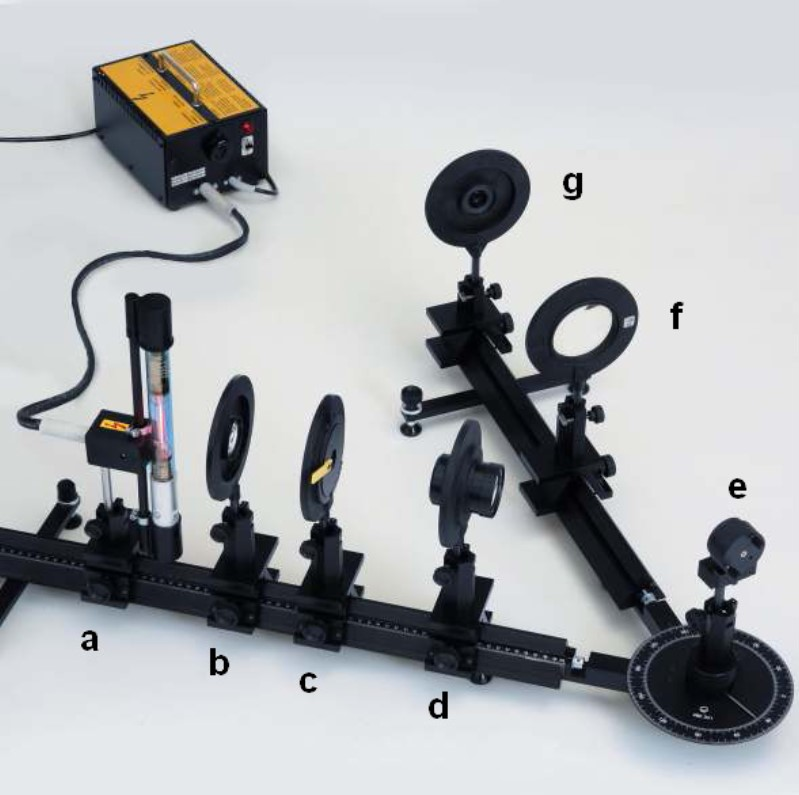
\includegraphics[width=0.5\textwidth]{balmer-aufbau}
  \caption{Aufbau zur Durchmessung der Balmer-Serie \cite{Anleitung}}
  \label{fig:balmer-aufbau}
\end{figure}
Die Linien sollen hier anhand einer Balmer-Lampe (a) beobachtet werden, welche herkömmliches sowie deuteriertes Wasser enthält.
Der Wasserdampf wird in der Lampe durch eine hohe Spannung zum Leuchten angeregt. Das Licht geht durch eine Linse (b), einen Spalt (c) 
und eine weitere Linse (d), welche als Projektionsobjektiv zur Kollimation dient, auf ein drehbar gelagertes Reflexionsgitter (e), welches hier als Interferometer dient. Das Muster kann an einer weiteren
drehbaren Schiene beobachtet werden, wo das Licht von einer weiteren Linse (f) auf das Okular (g) abgebildet wird.

Am Drehgelenk unter dem Gitter gibt es eine Winkelskala. Das Gitter wird zunächst auf \ang{0} gedreht und das Projektionsobjektiv in seinem Brennweitenabstand
(\SI{150}{\mm}, \cite{Anleitung}) hinter dem Spalt aufgestellt. Bei angeschalteter Lampe ist nun ein Bild des Spalts leicht neben dem Spalt zu sehen.
Damit das Gitter genau justiert ist, wird es in seiner Aufhängung so gedreht, dass das Bild des Spalts im Spalt selbst liegt.




\clearpage
\section{Fazit}


\clearpage
\begin{thebibliography}{9}

\bibitem{Anleitung}
\textit{Physikalisches Praktikum Teil IV -- Versuchsbeschreibungen}, Universität Bonn, 10.10.2024


\bibitem{demtröder3}
\textit{Experimentalphysik 3 -- Atome, Moleküle, Festkörper}, 5. Auflage, Wolfgang Demtröder, 2016


\end{thebibliography}

\end{document}

